\section{Experimental Results}
\subsection{Evaluation Metrics and Results}
To quantitatively evaluate the performance of our fraud detection framework, we computed several classification metrics derived from the confusion matrix. A confusion matrix summarizes classification results in terms of True Positives ($TP$), False Positives ($FP$), True Negatives ($TN$), and False Negatives ($FN$), providing insights into the model's capability to distinguish between fraudulent and legitimate transactions.

The confusion matrix obtained from our model predictions is illustrated in Figure~\ref{fig:confusion-matrix}.

\begin{figure}[h]
    \centering
    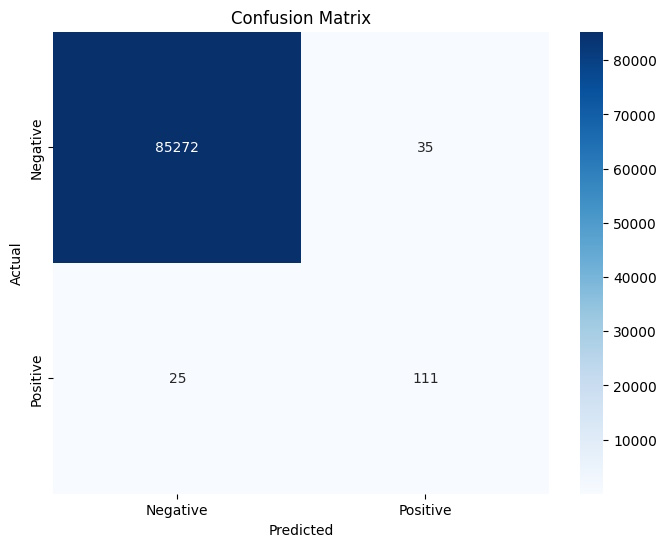
\includegraphics[width=0.8\linewidth]{images/confusion_matrix.jpg}
    \caption{Confusion Matrix of the Final Model}
    \label{fig:confusion-matrix}
\end{figure}

From this confusion matrix, we computed the following metrics:

\begin{itemize}
    \item \textbf{Precision}: The fraction of predicted fraudulent transactions that are correctly classified.
    \[
    \text{Precision} = \frac{TP}{TP + FP}
    \]

    \item \textbf{Recall} (Sensitivity): The fraction of actual fraudulent transactions correctly identified.
    \[
    \text{Recall} = \frac{TP}{TP + FN}
    \]

    \item \textbf{F1 Score}: The harmonic mean between Precision and Recall, providing a balanced metric.
    \[
    \text{F1 Score} = 2 \times \frac{\text{Precision} \times \text{Recall}}{\text{Precision} + \text{Recall}}
    \]

    \item \textbf{Accuracy}: The overall fraction of transactions correctly classified.
    \[
    \text{Accuracy} = \frac{TP + TN}{TP + TN + FP + FN}
    \]
\end{itemize}

The final classification results are summarized below:

\begin{itemize}
    \item Accuracy = $0.9993$
    \item Precision = $0.7603$
    \item Recall = $0.8162$
    \item Specificity = $0.9996$
    \item F1 Score = $0.7872$
\end{itemize}

These results demonstrate that our model effectively identifies fraudulent transactions while maintaining very high accuracy, highlighting its suitability for deployment in practical fraud detection scenarios.

\subsection{Discussion}
Our final classification model achieved strong performance metrics (Precision = $0.7603$, Recall = $0.8162$, F1-score = $0.7872$, Specificity = $0.9996$ and Accuracy = $0.9993$), demonstrating its capability to identify fraudulent transactions with a balanced combination of precision and recall. However, compared to the original results reported by Tayebi and El Kafhali~\cite{Tayebi2025} (Precision = $0.985$, Recall = $0.9705$, F1-score = $0.9777$, and Accuracy = $0.9999$), our model exhibited somewhat lower effectiveness in distinguishing fraudulent transactions, particularly in terms of precision and recall.

A key factor potentially contributing to this performance gap is our implementation of the autoencoder training phase. Specifically, the autoencoder's reconstruction quality for fraudulent transaction data was somewhat limited, resulting in synthetic samples with lower realism and variability. Consequently, the SVM filtering step discarded a significant portion of synthetic fraud samples, thereby restricting the size and diversity of our final training dataset. This limitation may have impacted the subsequent training and generalization capabilities of the ALSTM model.

To address this, future efforts could include enhancing the autoencoder's training procedure, such as experimenting with deeper architectures, varying the latent dimensions, or employing alternative regularization and data augmentation strategies. Such improvements may lead to higher-quality synthetic data generation and potentially bridge the observed performance discrepancy between our results and those of the original study.

\paragraph{Note on evaluation metrics computed in the original paper}
During the analysis of the model's performance, an inconsistency emerged concerning the definitions of evaluation metrics originally provided by the reference paper. Specifically, the definitions of \textbf{specificity} and \textbf{recall} were inverted compared to the commonly accepted standards in the literature. Using the formulas from the original paper, in our work, the newly computed specificity is $0.8162$ and recall is $0.9996$, resulting in an F1 Score of $0.8637$, which is significantly higher than the correct value of $0.7872$ obtained with standard definitions.
